\documentclass{utils/sig-alternate}
% \documentclass{utils/acm_proc_article-sp}

\usepackage[utf8]{inputenc}
\usepackage[T1]{fontenc}
\usepackage{textcomp}
\usepackage[english, french]{babel}
\usepackage{algorithm}
\usepackage{algpseudocode}
\usepackage{graphicx}
\usepackage{hyperref}
\usepackage{backnaur}

\usepackage{tikz}
\usepackage{pgfplots}
\usepgfplotslibrary{external} 
\tikzexternalize
\tikzsetexternalprefix{figures/}
\newcommand*\circled[1]{
  \tikz[baseline=(char.base)]{%
    \node[shape=circle,draw,inner sep=0.8pt] (char) {#1};
  }%
}


\usepackage[hyperref=true,%
            url=false,%
            isbn=false,%
            style=numeric,%
            maxcitenames=3,%
            maxbibnames=100,%
            backend=biber,%
            block=none]{biblatex}

\bibliography{../src/bib/OS.bib}
\bibliography{../src/bib/Flow-Based Programming.bib}
\bibliography{../src/bib/Functional Programming-Functional Reactive Programming.bib}
\bibliography{../src/bib/Stream.bib}
\bibliography{../src/bib/Dataflow.bib}
\bibliography{../src/bib/Web & Social Networks.bib}
\bibliography{../src/bib/Others.bib}
\bibliography{../src/bib/Actor Model.bib}
\bibliography{../src/bib/Misc.bib}
\bibliography{../src/bib/Parallelisation.bib}
\bibliography{../src/bib/Others.bib}
\bibliography{../src/bib/Distributed Systems.bib}
\bibliography{../src/bib/Compilation.bib}
\bibliography{../src/bib/MyPublications.bib}
\bibliography{../src/bib/Sync-Async.bib}
% \bibliography{../src/bib/sigproc.bib}

% \bibliographystyle{abbrv}
% \bibliography{../src/bib/OS.bib,../src/bib/Flow-Based Programming.bib,../src/bib/Functional Programming-Functional Reactive Programming.bib,../src/bib/Stream.bib,../src/bib/Dataflow.bib,../src/bib/Web & Social Networks.bib,../src/bib/Others.bib,../src/bib/Actor model.bib,../src/bib/Misc.bib,../src/bib/Parallelisation.bib,../src/bib/Others.bib,../src/bib/Distributed Systems.bib}

\usepackage{color}
\usepackage{listings}

% Configuration de la coloration syntaxique du code
\definecolor{bleugris}{rgb}{.2,.4,.5}
\definecolor{colKeys}{rgb}{0,0,1}
\definecolor{colIdentifier}{rgb}{0,0,0}
\definecolor{colComments}{rgb}{0,0.5,1}
\definecolor{colString}{rgb}{0.6,0.1,0.1}

\newcommand{\nClass}[1]{{\color{bleugris}{\textsl{\textbf{#1}}}}}
\newcommand{\nParameter}[1]{{\color{gray}{\textbf{#1}}}}
\newcommand{\nMethod}[1]{{\color{gray}{\textbf{#1}}}}
\newcommand{\nConstant}[1]{\texttt{\uppercase{#1}}}
\newcommand{\nKeyword}[1]{\textsl{\textbf{#1}}}


\definecolor{lightgray}{rgb}{.9,.9,.9}
\definecolor{darkgray}{rgb}{.4,.4,.4}
\definecolor{purple}{rgb}{0.65, 0.12, 0.82}
\lstdefinelanguage{JavaScript}{
  keywords={break, case, catch, continue, debugger, default, delete, do, else, false, finally, for, function, if, in, instanceof, new, null, return, switch, this, throw, true, try, typeof, var, void, while, with},
  morecomment=[l]{//},
  morecomment=[s]{/*}{*/},
  morestring=[b]',
  morestring=[b]",
  ndkeywords={class, export, boolean, throw, implements, import, this},
  keywordstyle=\color{blue}\bfseries,
  ndkeywordstyle=\color{darkgray}\bfseries,
  identifierstyle=\color{black},
  commentstyle=\color{purple}\ttfamily,
  stringstyle=\color{red}\ttfamily,
  sensitive=true
}

\newcommand{\userlstset}[1]{
  \lstset{ %
    language=#1,                   % choose the language of the code
    identifierstyle=\color{colIdentifier},%
    basicstyle=\ttfamily\scriptsize, %
    keywordstyle=\color{colKeys},%
    stringstyle=\color{colString},%
    commentstyle=\color{colComments},%
    numberstyle=\tiny,              % the size of the fonts that are used for the line-numbers
    numbers=left,                   % where to put the line-numbers
    stepnumber=1,                   % the step between two line-numbers. If it is 1 each line will be numbered
    numbersep=5pt,                  % how far the line-numbers are from the code
    backgroundcolor=\color{white},  % choose the background color. You must add \usepackage{color}
    showspaces=false,               % show spaces adding particular underscores
    showstringspaces=false,         % underline spaces within strings
    showtabs=false,                 % show tabs within strings adding particular underscores
    %frame=single,                  % adds a frame around the code
    tabsize=2,                      % sets default tabsize to 2 spaces
    captionpos=b,                   % sets the caption-position to bottom
    breaklines=true,                % sets automatic line breaking
    breakautoindent = true,         %
    breakatwhitespace=false,        % sets if automatic breaks should only happen at whitespace
    escapeinside={\@}{\@},         % if you want to add a comment within your code
    % texcl=true
  } %
}

\newcommand{\ic}[1]{\lstinline|#1|}

\lstnewenvironment{code}[1][JavaScript]{%
  \userlstset{#1}%
}{%
}
\usepackage{marginnote}
\usepackage{xcolor}

\definecolor{todo}{rgb}{0.9,0.5,0.5}
\definecolor{text}{gray}{0.8}

\newcommand{\TODO}[1]{%
	% \marginpar
	{
		\textcolor{todo}{\bf TODO}
		\textcolor{text}{#1}
	}
}

\newcommand{\ind }{%
  \hspace{4ex}%
}

\newcommand{\comment}[1]{%
  \textcolor{text}{#1}%
}

\newcommand{\nt}[1]{%
  \textcolor{red}{*}%
  \marginpar{\textcolor{red}{{\fontencoding{U}\fontfamily{futs}\selectfont\char 66\relax}}\vspace{3mm}\\
  \tiny{\textcolor{text}{#1}}}%
}

\newcommand{\ftnt}[1]{%
\footnote{\small{\url{#1}}}%
}

\newlength\callStackIndentation
\newcommand{\level}[1]{%
  \setlength\callStackIndentation{2em}%
  \hspace*{#1\callStackIndentation}%
}



\definecolor{red}{rgb}{1,0,0.29}
\definecolor{gray1}{rgb}{.70,.70,.70}
\definecolor{gray2}{rgb}{.75,.75,.75}
\definecolor{gray3}{rgb}{.80,.80,.80}
\definecolor{gray4}{rgb}{.85,.85,.85}
\definecolor{gray5}{rgb}{.90,.90,.90}
\definecolor{gray6}{rgb}{.95,.95,.95}

\makeatletter

\tikzstyle{chart}=[
    legend label/.style={font={\scriptsize},anchor=west,align=left},
    legend box/.style={rectangle, draw, minimum size=5pt},
    axis/.style={black,semithick,->},
    axis label/.style={anchor=east,font={\tiny}},
]

\tikzstyle{pie chart}=[
    chart,
    slice/.style={line cap=round, line join=round, very thick,draw=white},
    pie title/.style={font={\bf}},
    slice type/.style 2 args={
        ##1/.style={fill=##2},
        values of ##1/.style={}
    }
]

\tikzstyle{bar chart}=[
    chart,
    bar width/.code={
        \pgfmathparse{##1/2}
        \global\let\bar@w\pgfmathresult
    },
    bar/.style={very thick, draw=white},
    bar label/.style={font={\bf\small},anchor=north},
    bar value/.style={font={\footnotesize}},
    bar width=.75,
]

\pgfdeclarelayer{background}
\pgfdeclarelayer{foreground}
\pgfsetlayers{background,main,foreground}


\newcommand{\pie}[3][]{
    \begin{scope}[#1]
    \pgfmathsetmacro{\curA}{90}
    \pgfmathsetmacro{\r}{0.8}
    \def\c{(0,0)}
    % \node[pie title] at (90:1.3) {#2};
    \foreach \v/\s in{#3}{
        \pgfmathsetmacro{\deltaA}{\v/100*360}
        \pgfmathsetmacro{\nextA}{\curA + \deltaA}
        \pgfmathsetmacro{\midA}{(\curA+\nextA)/2}

        \path[slice,\s] \c
            -- +(\curA:\r)
            arc (\curA:\nextA:\r)
            -- cycle;
        \pgfmathsetmacro{\d}{max((\deltaA * -(.5/50) + 1) , .5)}

        \begin{pgfonlayer}{foreground}
        \path \c -- node[pos=\d,pie values,values of \s]{$\v\%$} +(\midA:\r);
        \end{pgfonlayer}

        \global\let\curA\nextA
    }
    \end{scope}
}

\newcommand{\legend}[2][]{
    \begin{scope}[#1]
    \path
        \foreach \n/\s in {#2}
            {
                  ++(0,-5pt) node[\s,legend box] {} +(3pt,0) node[legend label] {\n}
            }
    ;
    \end{scope}
}


% Document starts
\begin{document}

% Title portion
\title{
  Transforming Javascript event-loop into a scalable pipeline
	% Toward a compiler providing pipeline parallelism for the Javascript event-loop.
  % : hide scalability constraints from the developer
}

% \numberofauthors{4}
% \author{
% % 1st. author
% \alignauthor
% Etienne Brodu\\
%   \email{\textsf{\normalsize{etienne.brodu@insa-lyon.fr}}}\\
%   \affaddr{\textsf{\small{Université de Lyon, INRIA,}}}\\
%   \affaddr{\textsf{\small{INSA-Lyon, CITI-INRIA, F-69621, Villeurbanne, France}}}
% % 2nd. author
% \alignauthor
% Stéphane Frénot\\
%   \email{\textsf{\normalsize{stephane.frenot@insa-lyon.fr}}}\\
%   \affaddr{\textsf{\small{Université de Lyon, INRIA,}}}\\
%   \affaddr{\textsf{\small{INSA-Lyon, CITI-INRIA, F-69621, Villeurbanne, France}}}
% % \and  % use '\and' if you need 'another row' of author names
% % 3rd. author
% \alignauthor
% Frédéric Oblé\\
%   \email{\textsf{\normalsize{frederic.oble@worldline.com}}}\\
%   \affaddr{\textsf{\small{Worldline}}}\\
%   \affaddr{\textsf{\small{Bât. Le Mirage, 53 avenue Paul Krüger}}}\\
%   % \affaddr{\textsf{\small{CS 60195}}}\\
%   \affaddr{\textsf{\small{69624 Villeurbanne Cedex}}}\\
% }

\maketitle

\begin{abstract}

The development of a real-time web application often starts with a feature-oriented approach allowing to quickly react to users feedbacks.
However, this approach poorly scales in performance.
Yet, the audience can increase by an order of magnitude in a matter of hours. This first approach is unable to deal with the higher connections spikes.
It leads the development team to shift to a scalable approach often linked to new development paradigm such as dataflow programming.
This shift of technology is disruptive and continuity-threatening.
To avoid this shift, we propose to abstract the feature-oriented development into a more scalable high-level language.
Indeed, reasoning on this high-level language allows to dynamically cope with audience growth and decrease.

We propose a compilation approach that transforms a Javascript, single-threaded real-time web application into a network of small independent parts communicating by message streams.
We named these parts \textit{fluxions}, by contraction between a flow (flux in french) and a function.
The independence of these parts allows their execution to be parallel, and to organize an application on several processors to cope with its load, in a similar way network routers do with IP traffic.
% The dynamic reorganization of these parts in a cluster of machine can help an application to deal with its load in a similar way network routers do with IP traffic.
% \comment{it might be true, but it seems completely unrelated to me. Maybe because I don't understand IP enough}
We test this approach by applying the compiler to a real web application.
We transform this application to parallelize the execution of an independent part and present the result.

\end{abstract}

\endinput

% The very short abstract 50 words

Web applications starts with a feature-oriented approach to quickly react to users feedbacks, but eventually shift to a more scalable approach.
To avoid this disruptive shift, we propose an equivalence to compile the feature-oriented approach to a scalable high-level language.
We test this approach by applying the compiler to a real web application.


% A category with the (minimum) three required fields
% \category{H.4}{Information Systems Applications}{Miscellaneous}
%A category including the fourth, optional field follows...
% \category{D.2.8}{Software Engineering}{Metrics}[complexity measures, performance measures]

\category{Software and its engineering}{Software notations and tools}{Compilers}[Runtime environments]

\terms{Compilation, dataflow, code transformation}

\keywords{Flow programming, Web, Javascript} % NOT required for Proceedings

% \eject

\section{Introduction}

The growth of web platforms is partially due to Internet's capacity to allow very quick releases of a minimal viable product (MVP).
In a matter of hours, it is possible to release a prototype and start gathering a user community.
\textit{``Release early, release often''}, and \textit{``Fail fast''} are the punchlines of the web entrepreneurial community.
It is crucial for the prosperity of such project to quickly validate that the proposed solution meets the needs of its users.
Indeed, the lack of market need is the number one reason for startup failure.\ftnt{https://www.cbinsights.com/blog/startup-failure-post-mortem/}
That is why the development team quickly concretises an MVP using a feature-driven approach and iterates on it.

If the service successfully complies with users requirements, its community might grow with its popularity.
The service needs to be scalable to be able to respond to this growth.
However, feature-based development best practices are incompatible with the requirement of scalability.
The features are bundled in modules which spread through the code base.
This intertwining overlaps, hence disturbs the organization of a scalable execution.
Eventually this growth requires to discard the initial approach to adopt a more efficient processing model instead.
Many of the most efficient models distribute the system on a cluster of commodity machines \cite{Fox1997}.
MapReduce \cite{Dean2008} and the Staged Event-driven Architecture (SEDA) \cite{Welsh2000} are famous examples of that trend. %, using a pipeline architecture.
Once split, the service parts are connected by an asynchronous messaging system.
Many tools have been developed to express and manage these service parts and their communications.
We can cite Spark \cite{Zaharia2010}, MillWheel \cite{Akidau2013}, Timestream \cite{Qian2013}, Naiad \cite{McSherry} and Storm \cite{Toshniwal2014}, and many others.
However, these tools are in disruption from the initial approach.
It requires the development team either to be trained or to hire experts, and to start over the initial code base.
This shift causes the development team to spend development resources in background without adding visible value for the users.$^2$
It is a risk for the evolution of the project as the number two and three reasons for startup failures are running out of cash, and missing the right competences.
% \ftnt{https://www.cbinsights.com/blog/startup-failure-post-mortem/}

The risks described above comes from a disruption between the two levels of application expression, the feature level and the execution level.
To lift these risks, we propose a tool to identify the alignment between the two level, so as to allow a continuous transition from one to the other.
% This compiler transforms the initial code base into a high-level language.
% in the application allowing parallelism, hence scalability.
We focus on web applications driven by users requests, developed in Javascript using the \textit{Node.js} execution environment.

Javascript is increasingly used to develop web applications.
It is the most used language on Github\ftnt{http://githut.info/}, and StackOverflow\ftnt{http://stackoverflow.com/tags}.
We think that it is possible to analyze this type of application as a stream of requests, passing through a pipeline of stages.
Indeed, the event-loop used in \textit{Node.js} is very similar to a pipeline architecture.
We propose a compiler to transform a Javascript application into a network of autonomous parts communicating by message streams.
We named these parts \textit{fluxions}, by contraction between a flux and a function.
We are interested in the problems arising from the isolation of the global memory into these fluxions.
%This tool and its runtime aim not to modify the existing code, but rely on a high-level language expression over the initial code base.
We present an early version of this tool as a proof of concept for this compilation approach.
We start by describing in section \ref{section:model} the execution environment targeted by this compiler.
Then, we present the compiler in section \ref{section:compiler}, and its evaluation in section \ref{section:evaluation}.
We compare our work with related works in section \ref{section:related}.
And finally, we conclude this paper.
\section{Fluxional execution model} \label{section:model}

% The compiler we present in section \ref{section:compiler} focuses on web applications that tend to follow the functional paradigm while keeping a global memory.
% Such applications are built using functions that are executed sequentially to assure the exclusivity of access on the global memory.
% This is a serious performance issue, as it avoids to leverage the parallelism of modern architectures.

% We present in this section a different execution model that isolates the memory accessible to some functions.
% This approach allows to execute these functions in parallel, hence, to benefit of the performance improvements of this parallelism.
% This execution model is close to the actor model, as the function are executed on autonomous execution units with their own isolated memory, communicating by messages.

% In this section, we present an execution model to allow the execution of functions in parallel of a main thread.
% Each parallel function is encapsulated in an autonomous execution container with its own memory.

This section presents an execution model to provide scalability to web applications with a granularity of parallelism at the function level.
Functions are encapsulated in autonomous execution containers with their state, so as to be mobile and parallel, similarly to the actors model.
The communications are similar to the dataflow programming model, which allows to reason on the throughput of these streams, and to react to load increases \cite{Bartenstein2014}.
% This execution model is close to the actors model, as the execution containers are independent and communicate by messages.
% As we focus on real-time web applications, the streams of message correspond to the input stream of requests.

% This execution model is also close to the functional paradigm, as the execution container contains function to execute at each message reception.
% The function receives parameters from the input message, and sends one, or more, output streams of messages to other execution container.

The fluxional execution model executes programs written in our high-level fluxionnal language, whose grammar is presented in figure \ref{fig:flx-lang}.
An application $\bnfpn{program}$ is partitioned into parts encapsulated in autonomous execution containers named \textit{fluxions} $\bnfpn{flx}$.
The following paragraphs present the \textit{fluxions} and the messaging system to carry the communications between \textit{fluxions}, and then an example application using this execution model.

\subsection{Fluxions and Messaging System}
% $\bnfpn{flx}$
% $\bnfpn{id}$
% $\bnfpn{fn}$
% $\bnfpn{ctx}$
% $\bnfpn{fn}$
% $\bnfpn{stream}$
% $\bnfpn{dest}$

% The fluxional execution model manages and invokes fluxions.
A \textit{fluxion} $\bnfpn{flx}$ is named by a unique identifier $\bnfpn{id}$ to receive messages, and might be part of one or more groups indicated by tags $\bnfpn{tags}$.
A \textit{fluxion} is composed of a processing function $\bnfpn{fn}$, and a local memory called a \textit{context} $\bnfpn{ctx}$.
% Figure \ref{fig:flx-lang} presents the fluxionnal language we designed to express fluxions.
% The function encapsulated by a \textit{fluxion} consumes an input stream and generates one or more outputs streams.

At a message reception, the \textit{fluxion} modifies its \textit{context}, and sends messages to downstream \textit{fluxions} on its output streams $\bnfpn{streams}$.
The \textit{context} stores the state on which a \textit{fluxion} relies between two message receptions.
% The messaging system carries the stream communications between fluxions based on the names of the recipient fluxions.
% After the execution of a \textit{fluxion},
The messaging system queues the output messages for the event loop to process them later by calling the downstream \textit{fluxions}.
% A message is composed of the recipient fluxions' names and a body.
% Message passing is unable\footnote{at reasonable costs} to replace the synchronization allowed by shared state. % and required between some of the application parts.

In addition to message passing, the execution model allows \textit{fluxions} to communicate by sharing state between their \textit{contexts}.
% To allow this synchronization when required, the execution model allows fluxions to share state between their contexts.
The fluxions that need this synchronization are grouped with the same tag, and loose their independence.
% To assure the consistency of the shared state, all the fluxions of a group are executed sequentially.
% Though, the different groups of fluxions are executed in parallel.

There are two types of streams, \textit{start} and \textit{post}, which correspond to the nature of the rupture point producing the stream.
A variable created within a chain of \textit{post} streams requires more synchronization than a variable created upstream a \textit{start} stream.
The two types and implications of rupture points are further detailed in section \ref{section:compiler}.
% We differentiate the two types with two different arrows, double arrow (\texttt{>>})                         for \textit{start} rupture points and simple arrow (\texttt{->})          for \textit{post} rupture points.
\textit{Start} rupture points are indicated with a double arrow ($\to$ \hspace{-1.4em} $\to$ or \texttt{>>}) and \textit{post} rupture points with a simple arrow ($\to$ or \texttt{->}).


% It is the target for our compiler.
\begin{figure}[h]
\vspace{-0.6\baselineskip}
\begin{bnf*}
  \bnfprod{program}    {\bnfpn{flx} \bnfor \bnfpn{flx} \bnfsp \bnftd{eol} \bnfsp \bnfpn{program}}\\
  \bnfprod{flx}        {\bnfts{\texttt{flx}} \bnfsp \bnfpn{id} \bnfsp \bnfpn{tags} \bnfsp \bnfpn{ctx} \bnfsp \bnftd{eol} \bnfsp \bnfpn{streams} \bnfsp \bnftd{eol} \bnfsp \bnfpn{fn}}\\
  % \bnfprod{tags}       {\bnfts{\bnfpn{id}} \bnfor \bnfpn{id} \bnfsp \bnftd{eol} \bnfsp \bnfpn{tags} \bnfor \bnftd{empty string}}\\
  \bnfprod{tags}       {\bnfts{\texttt{\&}} \bnfsp \bnfpn{list} \bnfor \bnftd{empty string}}\\
  \bnfprod{streams}    {\bnfts{\texttt{null}} \bnfor \bnfpn{stream} \bnfor \bnfpn{stream} \bnfsp \bnftd{eol} \bnfsp \bnfpn{streams}}\\
  \bnfprod{stream}     {\bnfpn{type} \bnfsp \bnfpn{dest} \bnfsp [\bnfpn{msg}]}\\
  \bnfprod{dest}       {\bnfpn{list}}\\
  \bnfprod{ctx}        {\bnfts{\texttt{\{}} \bnfpn{list} \bnfts{\texttt{\}}}}\\
  \bnfprod{msg}        {\bnfts{\texttt{[}} \bnfpn{list} \bnfts{\texttt{]}}}\\
  \bnfprod{list}       {\bnfpn{id} \bnfor \bnfpn{id} \bnfsp \bnfts{,} \bnfsp \bnfpn{list}}\\
  \bnfprod{type}       {\bnfts{\texttt{>}\texttt{>}} \bnfor \bnfts{\texttt{-}\texttt{>}}}\\
  \bnfprod{id}         {\bnftd{Identifier}}\\
  \bnfprod{fn}         {\bnftd{Source language with~} \bnfpn{stream} \bnftd{~placeholders}}\\
\end{bnf*}
\vspace{-2.5\baselineskip}
\caption{Syntax of a high-level language to represent a program in the fluxionnal form}
\label{fig:flx-lang}
\end{figure}

% Fluxions are executed on an event-loop with an isolated heap ; it is a \textit{Node.js} instance.
% We propose to stretch the execution of an application by distributing the fluxions on different event-loops.
% But the distribution is limited by the dependencies between fluxions.
% All the fluxions of a group need to be gathered on the same event-loop.
% Indeed, each event-loop assures the exclusivity of access to the state: only one fluxion is executed at once.
% Consequently, the more fluxions are gathered on an event-loop, the less time fraction each fluxion can use without impacting the throughput.

%These groups represent the graph of state communications between fluxion.
%Hence, this graph indicates the states that are limiting the parallelism.


% A fluxion receiving and sending heap reference can be stateless, hence replicated.
% However, because it share references, it needs to be on the same group than other another fluxions (think about req / res).
% If all the fluxion of a group are stateless, they can be replicated exactly like if it was a single fluxion. 





% \subsection{Messaging system}

% In a distributed approach, the messages between fluxions would be carried over a distributed message broker.
% However this execution model is only a simulation of a distributed execution environement.
% We simplify the distributed message broker with a master message queue to centralize communication between workers, though, each worker has its own local message queue.
% The messaging system is the core of the execution model.
% It carries messages and invokes fluxions at reception.
% The messaging system sends messages to the worker hosting the destination fluxion.
% Locally, the master worker hosts fluxions that need access to the external network or the global memory.
% Using a message queue allows to execute multiple processing chains fairly and concurrently, without difference in scheduling local messages, or network messages.

% The messages are queued for the event-loop to execute the associated fluxions sequentially.

% The execution model allows each group of fluxions to be executed on a remote event-loop.
% Therefore, some messages need to be send to remote event-loops.
% When processing a message, if the destination fluxion is local, the messaging system immediately invokes the fluxion with the message, if it is on a remote event-loop, the messaging system sends the message to be queued on the remote event-loop.



% The messaging system carries messages from one event-loop to the other, and assure that the message is queued on the event-loop executing the destination fluxion.

% If two fluxions share the same name, it would lead to a conflicting situation for the messaging system.

% This registration associates a processing function with a unique name and an initial \textit{context}.
% The registration is done by calling \texttt{register(<name>, <fn>, <context>)}, \circled{1}.
% A fluxion can dynamically register other fluxions

% \nt{the example in figure 2 is only partially explained in text, many parts (group network, program, enqueue...) are not explained.}

% Algorithms \ref{alg:parcours} and \ref{alg:traitement} describe the behavior of the messaging system after the \texttt{start} function invocation.

% \begin{algorithm}
% \caption{Message queue walking algorithm}
% \label{alg:parcours}
% \begin{algorithmic}
% \Function{loopMessage}{\null}
% \While{$msg$ \textbf{presents in} $msgQueue$}
% \State $msg \gets$ \Call{dequeue}{\null} \Comment{\circled{3}}
% \State \Call{ProcessMsg}{$msg$}
% \EndWhile
% \EndFunction
% \end{algorithmic}
% \end{algorithm}

% \begin{algorithm}
% \caption{Message processing algorithm}
% \label{alg:traitement}
% \begin{algorithmic}
% \Function{processMsg}{$msg$}
% \For{$dest$ \textbf{in} $msg.dest$}
% \State $worker \gets lookup(dest)$
% \State \Call{worker.send}{$fluxion, msg.body$} \Comment{\circled{4}}
% % \State $message \gets$ \Call{exec}{$fluxion, msg.body$} \Comment{\circled{4} \& \circled{5}}
% % \State \Call{enqueue}{$message$} \Comment{\circled{6}}
% \EndFor
% \EndFunction
% \end{algorithmic}
% \end{algorithm}

\subsection{Example}

\begin{code}[js,
  caption={Example web application},
  label={lst:source}]
var app = require('express')(),
    fs = require('fs'),
    count = 0; //@\label{lst:source-counter}@

app.get('/', function handler(req, res){ //@\label{lst:source-handler}@
  fs.readFile(__filename, function reply(err, data) {
    count += 1;
    res.send(err || template(count, data)); //@\label{lst:source-send}@
  });
}); //@\label{lst:source-handler-end}@

app.listen(8080);
\end{code}

The fluxional execution model is illustrated with an example application presented in listing \ref{lst:source}.
This application reads a file, and sends it back along with a request counter.
The \texttt{handler} function, line \ref{lst:source-handler} to \ref{lst:source-handler-end}, receives the input stream of requests.
The \texttt{count} variable at line \ref{lst:source-counter} counts the requests, and needs to be saved between two messages receptions.% in the fluxion \textit{context}.
The \texttt{template} function formats the output stream to be sent back to the client.
The \texttt{app.get} and \texttt{res.send} functions, lines \ref{lst:source-handler} and \ref{lst:source-send}, interface the application with the clients.
Between these two interface functions is a chain of three functions to process the client requests : \texttt{app.get} $\to$ \hspace{-1.4em} $\to$ \texttt{handler} $\to$ \texttt{reply}.
This chain of functions is transformed into a pipeline, expressed in the high-level fluxionnal language in listing \ref{lst:fluxional}.
The transformation process between the source and the fluxional code is explained in section \ref{section:compiler}.

\begin{figure}[h!]
  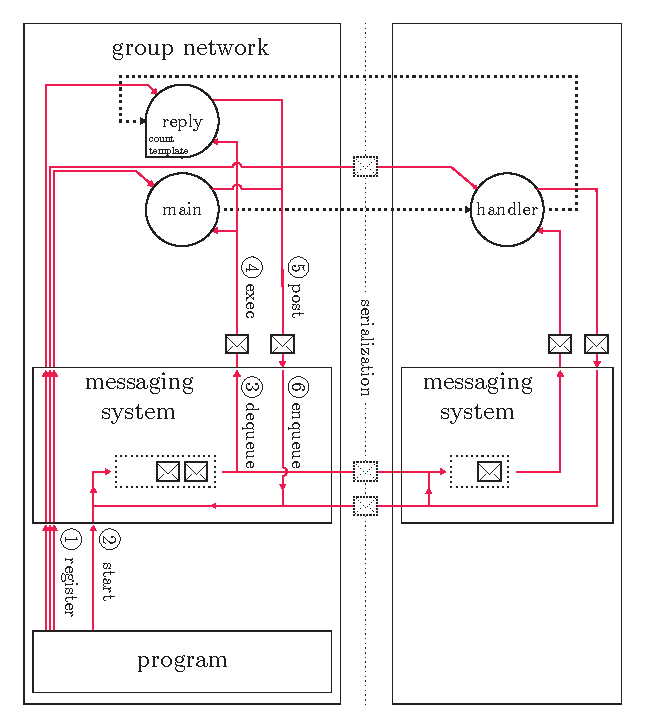
\includegraphics[width=\linewidth]{ressources/schema-message.pdf}
  \caption{The fluxionnal execution model in details}
  \label{fig:MesSys}
\end{figure}

The execution is illustrated in figure \ref{fig:MesSys}.
The dashed arrows between fluxions represent the message streams as seen in the fluxionnal application.
The plain arrows represent the operations of the messaging system during the execution.
These steps are indicated by numeroted circles.
% In the execution cycle of the example, illustrated in figure \ref{fig:MesSys}, numeroted circles indicate the step in the execution.
% The bigger circles represent the registered fluxions.
The \textit{program} registers its fluxions in the messageing system, \circled{1}.
The fluxion \textit{reply} has a context containing the variable \texttt{count} and \texttt{tem\-plate}.
% The streams between workers are serialized.
% To assure the consistency of their shared contexts, all the fluxions grouped with the same tag are executed sequentially and share the same message queue.
% Though, the different groups of fluxions are executed in parallel with different event queues.
% This first message represents the incoming of a request from a user.
When the application receives a request, the first fluxion in the stream, \textit{main}, queues a \texttt{start} message containing the request, \circled{2}.
This first message is to be received by the next fluxion \textit{handler}, \circled{3}, and triggers its execution, \circled{4}.
The fluxion \textit{handler} sends back a message, \circled{5}, to be enqueued, \circled{6}.
The system loops through steps \circled{3} through \circled{6} until the queue is empty.
This cycle starts again for each new incoming request causing another \texttt{start} message.

% The original source code of this application is available in listing \ref{lst:source}\footnote{The listings are also available on github\cite{flx-example}.}.
% In this example application, some points are worth noticing.

% We expect a similar result with the compiler described in section \ref{section:compiler}.
% Horizontal dashed lines show virtual transmission of messages between fluxions although they all go through the messaging system.

% \begin{figure}[h!]
%   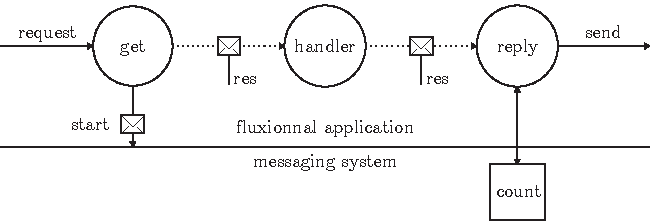
\includegraphics[width=\linewidth]{ressources/flux.pdf}
%   \caption{Fluxions chain manually extracted from the example application}
%   \label{fig:fluxions}
% \end{figure}

\begin{code}[flx, caption={Example application expressed in the high-level fluxional language}, label={lst:fluxional}]
flx main & grp_res
>> handler [res]
  var app = require('express')(),
      fs = require('fs'),
      count = 0;

  app.get('/', >> handler); //@\label{lst:fluxional-streamtohandler}@
  app.listen(8080);

flx handler
-> reply [res]
  function handler(req, res) {
    fs.readFile(__filename, -> reply); //@\label{lst:fluxional-readfile}@
  }

flx reply & grp_res {count, template}
-> null
  function reply(error, data) {
    count += 1; //@\label{lst:fluxional-counter}@
    res.send(err || template(count, data)); //@\label{lst:fluxional-ressend}@
  }
\end{code}

% The application is organized as follow.
The chain of functions from listing \ref{lst:source} is expressed in the fluxional language in listing \ref{lst:fluxional}.
% The stream of requests is received from the clients by the fluxion \texttt{main}, it continues in the fluxion \texttt{handler}, and finally goes through the fluxion \texttt{reply} to be sent back to the clients.
The fluxion \texttt{handler} doesn't have any dependencies, so it can be executed in a parallel event-loop.
The fluxions \texttt{main} and \texttt{reply} belong to the group \texttt{grp\_res}, indicating their dependency over the variable \texttt{res}.
The group name is arbitrarily chosen by the compiler.
% The last fluxion, \texttt{reply}, depends on the variable \texttt{res} created by the first fluxion, \texttt{main}.
% This variable is carried by the stream through the chain of fluxion to the fluxion \texttt{reply} that depends on it.
% The group \texttt{network} depends on this variable because it holds the references to the network sockets.
All the fluxions inside a group are executed sequentially on the same event-loop, to protect against concurrent accesses.

The variable \texttt{res} is created and consumed within a chain of \textit{post} stream.
Therefore, it is exclusive to one request and cannot be propagated to another request.
It doesn't prevent the whole group from being replicated.
However, the fluxion \texttt{reply} depends on the variable \texttt{count} created upstream the \textit{start} stream, which prevents this replication.
If it did not rely on this state, the group \texttt{grp\_res} would be stateless, and could be replicated to cope with the incoming traffic.

This execution model allows to parallelize the execution of an application as a pipeline, as with the fluxion \texttt{handler}.
And some parts are replicated, as could be the group \texttt{grp\_res}.
This parallelization improves the scalability of the application.
Indeed, as a fluxion contains its state and expresses its dependencies, it can be migrated.
It allows to adapt the number of fluxions per core to adjust the resource usage in function of the desired throughput.

Our goal, as described in the introduction, is not to propose a new high-level language but to automate the architectural shift.
We present the compiler to automate this architectural shift in the next section.

% \nt{I would also suggest adding labels to one of the fluxions in listing 2 to indicate its tags, context, steams and function.}

\section{Compiler} \label{section:compiler}

The first section of this paper describe the fluxionnal execution model, a framework to run web application in a distributed environment.
This section explains a method we developed to transform a subset of classic web application to be compliant with the execution model previously described.
This transformation unveils two problems due to the differences between a web application and the execution model.
In the first section, a distributed system is defined by the parallel execution of its parts, and the distribution of its memory.
A classic web application is not composed of many independent parts, and relies on a central memory.
The problems are to parallelize the execution of a mono-thread application into many parts, and to distribute the central memory among these independent parts.
\TODO{does it need a definition of the classic web application ? if so, should be in the introduction, not here}
We describe a compiler as a solution to this problems, hence capable to turn a classic web application into a scaling distributed system. \TODO{scaling is a bold claim, need some background}

The parallelization of a program designed for a mono thread architecture is a trending problem since the multiplication of the number of cores available on a machine.\TODO{references, see parallelization in my biblio}
It would allow developers to continue design application the same way they used to, while leveraging the performance of a multi-core architecture.
% Asynchronism is different than parallelism, but in certain cases, one allow the other.
From the sun programming guide\footnote{http://docs.oracle.com/cd/E19455-01/806-5257/6je9h032b/index.html}, parallelism is \textit{a condition that arises when at least two threads are executing simultaneously}, and concurrency is \textit{a condition that exists when at least two threads are making progress. A more generalized form of parallelism that can include time-slicing as a form of virtual parallelism}.
Asynchronism is a condition that arises during a communication, when a point doesn't wait for the answer to his request to continue processing an independent thread of execution.
In an asynchronous execution, the requested operation run along the main thread until the value is needed, releasing the main thread from waiting the operation to complete.
Promises\cite{Liskov1988} and Futures[??] are abstractions from an imperative, synchronous programing style, to an asynchronous execution model.
They transform synchronous, long waiting operations - like remote procedure calls or input output operations - into asynchronous operations.
% In a synchronous execution, the requested operation block the main thread until computation completes.
This asynchronism make the two execution paths independent, thus they can run in parallel until they are not independent enough - when one needs results from another.
We call rupture points, points where the execution flow forks in two independent and parallel paths.
These points mark out the limits between independent parts.

\TODO{next paragraph is a draft, needs rewrite}
Javascript is a functional and dynamically typed language initially introduced to handle user interactions within Web pages.
While Javascript isn't natively event-based, the DOM used in Web pages is.
The latter uses an event-loop to handle events happening on the Web page, and then triggers associated functions the developer provides.
\TODO{libevent, nginx : cite papers}
\TODO{references to interruptions}
More recently, \textit{Node.js} used the same event-loop based structure, to propose a non-blocking, event-based Javascript execution environment, specifically adapted for real-time I/O intensive applications like Web services.
Because of this event-loop based architecture, the I/O API \textit{Node.js} provides is non-blocking and asynchronous.
% The invocation of any function from this API returns immediately not to block the execution with time consuming I/O operations.
The developer provide an handler function as argument for this asynchronous function to invoke when the operation completes.
This handler function is commonly named a callback.%, \textit{Node.js} uses the convention to place the callback as the last parameter.
The \textit{Node.js} event-loop receives and gathers every I/O event, waiting its turn in the loop to invoke the associated callback.
% Listing \ref{lst:callback} illustrates the call of the asynchronous function \texttt{asyncFn} with the callback \texttt{callbackFn}.
% In most imperative languages the execution is synchronous by default, while special libraries handle parallelism, some using asynchronism like Promises and Futures cited above.
% However, 
\textit{Node.js} imposes natively an asynchronous paradigms along with the classic synchronous execution flow.
An asynchronous functions split the execution along two concurrent execution paths, the path independent from the asynchronous request, and the path handling the answer of the request.
We defined rupture points in \textit{Node.js} as an asynchronous function call using a callback mechanism to handle the result.
The two distinct execution paths are the synchronous instructions following the asynchronous function call, and the callback.
A rupture point marks out two independent parts of a web application.
One of the compilation step, the analyzer, spot the rupture points for the another compilation step, the mapper, to split the application along them.

\TODO {References of solutions to split memory into distributed parts ?}
Parallelism is not sufficient for an application to be distributed, because of the central memory.
Promises and Futures don't transform a central memory into a distributed memory.
\textit{Node.js} provide a central memory, while the execution model expect it to be distributed into the application parts.
The compiler needs to split the shared memory into the application parts for the application to be compliant with the execution model previously described.

In Javascript, scopes are nested one in the other, the parent being the global scope.
Each function create a new scope containing variables local to itself.
This scope is chained to the scope of the parent function, so that the child function can access variables in the scope of the parent function, up to the global scope.
Callbacks defined inside a scope can access the same scope as the calling function, allowing them to share variables.
% This feature is named closure.

Rupture points are always situated along scopes limits.
A scope is never shared between two application parts.
However, a child scopes separated in another application parts than its parent can't access the scopes it expects.
If the two scopes don't share the same memory, variables from the parent are unavailable for the child.
Another compiler step, the linker, understand and resolve dependencies conflicts between the distributed functions scopes.

In the next subsections, we describe the compilation steps.
Some part of the compilation chain are tools from the community, they are described in the first subsection along with the trivial compilation step.
Then, we describe three important compilation steps relevant to the two previously described problems.
The \textit{analyzer} detects rupture points in an application, later for the \textit{mapper} to break the application into many independent parts along the rupture points, then the \textit{linker} resolves inconsistencies between the shattered memory scopes.

\subsection{Common tools : parser and code generation}

The first compilation step is to parse the source code taken as input.
The last compilation step is to output Javascript code either as a Javascript source code to run on the fluxionnal execution model, or as code in another high-level langage describing the fluxions and their content.
Parsing code and generating code back are common tasks.
There exist community projects to fulfill these tasks, like \textit{Esprima} and \textit{Acorn}, two Javascript parser.
For this compiler we use a serie of tool written by Ariya Hidayat and Yusuke Suzuki for the projects \textit{Esprima} and \textit{Esmangle}.
These tools follow the specification for an intermediate representation of the Javascript source code from the Mozilla Javascript Parser API : the Abstract Syntax Tree (AST)\footnote{\raggedright https://developer.mozilla.org/en-US/docs/Mozilla/Projects/SpiderMonkey/Parser\_API}.
This structured representation breaks the source into a tree of nodes, each representing a construct from the source, like an operation or an identifier.
It can be traversed and allow easy modification of its structure, without the risk of errors involved by direct source manipulation.

An example node in the AST is :

\begin{code}[Javascript, caption={Example of an AST node},label={lst:astnode}]
CallExpression {
    type: "CallExpression";
    callee: <Expression>;
    arguments: [ <Expression> ];
}
\end{code}

The compiler uses \textit{Esprima} to parse the source and generate the AST.
It is the first compilation step.
Thes AST can be traversed and explore with the use of \textit{Estraverse}.
\textit{Escope} detects function scopes and variables declaration using the previously generated AST, and output an object to represent the organization of these scopes inside the source code.
One of the last compilation step is to produce a Javascript executable which uses the fluxionnal execution model.
To generate this Javascript code, the compiler use Escodegen, to transform back the AST into Javascript source code.

\subsection{Analyzer : spotting the rupture points}

The analyzer detects rupture points.
A rupture point is composed of an asynchronous function, and a callback.
We define in this section what a rupture point is, and how we detect them.

\subsubsection{Rupture points}

Rupture points are an asynchronous continuity in the execution flow, indicated by calls of asynchronous function with a callback in the parameters.
We distinguish specials rupture points indicated by asynchronous functions handling series of external requests, from basic rupture points indicated by asynchronous functions handling only a one time event inside of the application.
We distinguish these two types of rupture points to simplify later the dynamic analysis of the system load.
The special rupture points are the entry point for the flow of request, and so is a point of choice to measure the load during run-time.
We explain this point in details in the next section of this paper. \TODO{if we have the time to make the analysis}
% In a special rupture point, each new incoming request represent an additional load for the system.
% While the incoming request load is taken into account, the load of every application part following in the continuity of the execution flow can be infered before run-time. 
% The system load is only dependent at run time of the input in the system, everything else can be infered before run-time.
These two types of rupture points corresond to different asynchronous functions in the \textit{Node.js} I/O API : the functions handling only one I/O event, or a bounded series of I/O events, and the functions handling an unbounded serie of I/O events.

\paragraph{One-time event} \label{sss:post}

Basic rupture points are indicated by asynchronous functions providing immediate I/O operation.
Callbacks of these functions are invoked only once, and continue the execution after the completion of the I/O operation.
Because of their asynchronism, these function calls mark the frontier between the current application part and the next one, inside a chain of fluxion.
The rupture point is placed before the call to the asynchronous function, but after the resolution of the arguments.
The javascript middleware printer replaces the asynchronous function call by a call to a placeholder function.
% This placeholder function uses the function \texttt{post(<msg>)} provided by the fluxionnal execution model described section \ref{section:model}.
% The placeholder function is detailed later, section \ref{ss:Scope}.

\paragraph{Series of events} \label{sss:start}

Special rupture points are indicated by asynchronous functions providing a callback for a series of future event.
For example, the handler of a network socket is called once for each incoming request.
The callbacks of these functions indicate the input of a data stream in the program, and the beginning of a fluxions chain.
As the callbacks mark the frontier between the current fluxion and the beginning fluxions chain, the compiler replaces the callback by a placeholder function starting the chain.
% This placeholder function uses the function \texttt{start(<msg)} provided by the fluxionnal execution model described section \ref{section:model}.
% The placeholder function is detailed later, section \ref{ss:Scope}.

\subsubsection{Detection}

To detect a rupture point, it require to detect successfully the two components : the asynchronous function and the callback function.

\paragraph{Asynchronous functions}

Asynchronous functions are detected from their call name, linked from the module exposing them.
In Javascript, modules are included and stored in variables via the call to the \texttt{require} function.
The name of the variable holding the module is specified by the developer, so the only constant hold onto the asynchronous function is the call to the \texttt{require} function
The compiler uses a dictionnary of known asynchronous functions in modules to detect rupture points during the static analysis.
Such modules are \textit{Express} and \textit{fs}.
To find possible rupture points, the compiler tests the callee expression against the variable known for holding these modules.

To accurately detect the asynchronous function, we need to track the variables holding asynchronous functions.
The more accurately we can track changes in this variables, the more rupture points we can find, the better the application can be distributed.
This detection is done by traversing the AST, to find the node responsible for the assignment of modules in variables.
More advanced tracking technique could be used later to improve the efficiency of the compiler.


% The compiler detects one rupture point for the following hello world web application. 

% \begin{code}[Javascript, caption={Hello World},label={lst:hello}]
% var app = require('express');
% app.get('/', function(req, res) {
%   res.send("Hello World :)");
% });
% \end{code}

% TODO insert the graph for this program

% There is in this program only two scopes, the global scope, and the scope of the anonymous function.
% These two scopes don't share any variable.


\paragraph{Callback function}

To detect a callback function, we track every argument of an asynchronous function call to test if it is a function.
Some callback functions are declared \textit{in situ}, and are trivially detected.
For every other variable identifier, we track the declaration to recursively test the initialization value.
This method is not exhaustive, but it is a first step to increase the detection of rupture points.


\subsection{Mapper : correspondence between function scope and fluxion}

% The rupture points placed by the analyzer delimit all the application parts.

% A scope contains identifiers which are used as references to variables.
% These variables can be in the same scope than the identifier, or in any parent scope.
% That means an identifier and the refereed variable might be in different application parts, therefor, separated once the application is distributed.
% The mapper link every scope to the application part it is in, later for the Linker to be able to resolve unmet dependencies between scopes in different application parts.


% A rupture points is composed of two things : the asynchronous call, and the callback.
% The asynchronous call marks the execution limit between two application parts.
% The execution before and after the asynchronous call, the execution belong to a first application part.
% The execution of the asynchronous callback belongs to a second application part.
% The execution of the asynchronous function belonging depends of the type of the rupture point, determined by the type of the asynchronous function.

% The callback marks the scopes limit between two parts.
% The calling function's scope, and the callback function's scope belong in two different application parts.

% The callback might not be defined in the same scope as the asynchronous function, and might even be completely independent, relayed by assignation from one scope to another.
% To map the scopes to application parts, we must follow the callback limits : we enter a new application parts when we encounter a function flagged as a rupture point.

% However, application parts connectivity, by sending message occurs around the other component of a rupture point : the asynchronous function call.
% During this call, we send a message for the next application part to receive.


% Breaking the program.

The mapper breaks the program along rupture points to create application parts, later for these parts to be enclosed in fluxions as described in the previous section.
The two types of rupture points break differently.
The basic rupture point is an asynchronous continuity in the execution flow, it breaks before the asynchronous call, but after the resolution of the arguments.
\TODO{Why does it makes sense to include the asynchronous call in the next fluxion ?}

The special rupture point is an entry point into the system, making the system reacts for every request.
The asynchronous function of this type of rupture point is called one time, while the callback handling the event is triggered for each event.
That means the application parts containing the asynchronous function is executed one time, while the parts containing the callback is executed multiple times.
They cannot be in the same application parts, and be broken apart into two fluxions.



% There is two types of rupture points, and two type of situation for the callback definition.
% Rupture point can be of type start or post.
% The callback function can be declared anonymously, or not.
% As we are going to tamper with the code, we need to make the safest assumptions possible.
% If a function isn't anonymously declared in situ, there is chances it is used elsewhere, we need to be sure it is not the case before splitting the program into parts.

% To do that, we track the identifier used to pass the function in every scope it is accessible : the scope it is declared in, and every child scope.

% We encounter a limitation here.
% Because of conditional execution, we can't be sure of the alteration of a variable, and of its final value.
% We consider only the safest assumptions, so if an identifier is used beside its declaration, we assume the function it is referring to is used, and we can't simply remove it from the scope.




% \TODO{what about member expressions like handlers.event1}






\subsection{Linker : resolving dependencies} \label{ss:linker}

% In this example web application, the two fluxions share a common variable : \texttt{rep}.

% \begin{code}[Javascript, caption={Hello World with a shared variable},label={lst:sharedhello}]
% var app = require('express'),
%     rep = "Hello World :)";
% app.get('/', function(req, res) {
%   res.send(rep);
% });
% \end{code}

According to Brewer's theorem, formalized by Seth Gilbert and Nancy Lynch \cite{Gilbert2002}, a distributed application can only have two among the three options, Consistency, Availability, Partition tolerance.
As Coda Hale explained in one of his blog post\footnote{http://codahale.com/you-cant-sacrifice-partition-tolerance/}, network and node failures are unavoidable, a distributed system can't avoid to have failure.
Mike Stonebraker explain in another blog post\footnote{http://voltdb.com/blog/voltdb-products/clarifications-cap-theorem-and-data-related-errors/} that the trends is to make big data applications run on larger cluster of unreliable commodity machines.
Partition tolerance can't be avoided, so the only possible trade off is between consistency and availability.
These two tradeoff are defined in the literature as ACID (Atomicity, Consistency, Isolation, Durability) for consistency over availability, and BASE (Basically Available, Soft state, Eventual consistency) for availability over consistency.

If this trends is verified, transactional systems trading off availability for consistency might suffer from slower and slower response time, because of the rigidity of the requirements.
Choosing to sacrifice consistency might improve performance, because of the flexibility allowing to cope with problems emerging from highly distributed architecture, without durable inconsistency in the data because they are avoided by different synchronization techniques.
Amazon Dynamo system\cite{DeCandia2007} already demonstrated that these techniques can successfully be used to build a distributed system favoring availability without loosing consistency.
In the article presenting Amazon Dynamo system, the authors said that \textit{experience at Amazon has shown that data stores that provide ACID guarantees tend to have poor availability. This has been widely acknowledged by both the industry and academia}
This citation take reference from another paper\cite{Fox1997} where Eric Brewer is one of the author.

From the Amazon Dynamo system paper : 
``Dynamo uses a synthesis of well known techniques to achieve scalability and availability: Data is partitioned and replicated using consistent hashing\cite{Karger1997}, and consistency is facilitated by object versioning\cite{Lamport1978}. The consistency among replicas during updates is maintained by a quorum-like technique and a decentralized replica synchronization protocol. Dynamo employs a gossip based distributed failure detection and membership protocol. Dynamo is a completely decentralized system with minimal need for manual administration. Storage nodes can be added and removed from Dynamo without requiring any manual partitioning or redistribution''.

We use these papers to justify our choice for the linker to favor availability over consistency.
We believe we can make use of this well-known technique in the execution model.
As these techniques are already well-known, we focused our work on different problematics.

In the following section, we explain the different cases of inconsistency emerging from the partitioning of a central memory.
The linker analyzes how scopes are distributed among the application parts, and which variables are distributed on multiple application parts.
\textit{Escope} gives the compiler informations about the references of every variables in the application.
Among these references, we track the modifications of variables.

To resolve the dependencies in a fluxion's signature, the compiler uses different techniques.
\begin{description}
\item[Signature] If the variable is needed read-only by a downstream fluxion, it is sent following the message chain, from the upstream to the downstream fluxion.
\item[Scope] If the variable is modified by one fluxion, the variable is placed in the own memory of the application part, called scope. 
\item[Sync] If the variable is modified by at least two fluxion, the variable is synchronized between these fluxions.
\end{description}


\subsubsection{Signature}

  The variables needed for read-only access by one of the scope of a fluxion and modified by another fluxion represent its signature.
  The signature of a fluxion is added in the message body between two fluxions.
  The code inside the application part is modified to shift the corresponding references to point to the message.
  % Every reference of this variable is replaced by a reference pointing in the signature part of the message.
  % (basically reference -> msg.\_sign.reference)
  % As a fluxion is only called on a message reception, the variable should never be lacking.
  % If there is a problem in this situation, it is most likely a compilation error : the reference has not been replaced correctly, or the code is a corner case the compiler can't resolve yet.

\subsubsection{Scope}

  The own memory of an application parts holds the variables needed for modification, and never modified in another application part.
  This memory is stored in the scope of the fluxion encapsulating the application part.
  If one of this variables is needed for read by another fluxion downstream, this variable become part of the signature of the downstream fluxion.

\subsubsection{Sync}

  If a variable is needed for modification by more than one fluxion, this variable needs to be synchronised between the fluxions' scopes.
  In this context, we use techniques described earlier to reach eventual consistency.


% As fluxions are chained one after another, a fluxion must provide every dependency for the next one, even if some of this dependencies miss from its own scope or signature.
% These dependencies must be passed fluxion after fluxion from the producing fluxion, to the consuming fluxion.
% So, the message stream linking one fluxion to another includes the signature of the next fluxion as well as dependencies targeting downstream fluxions.
% The compiler has to resolve the content of these message streams beginning by the last fluxions and going upstream to the first ones.
% Figure \ref{fig:streamline} illustrate this principle : since fluxion \textit{C} needs the variable \textit{z}, fluxion \textit{B} needs the variable \textit{z} as well to pass it along to fluxion \textit{C}.

% \begin{figure}[h!]
%   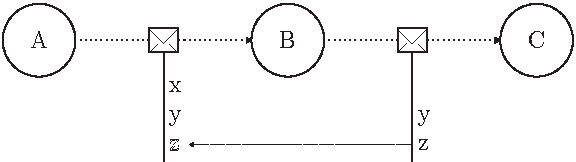
\includegraphics[width=\linewidth]{ressources/streamline.pdf}
%   \caption{Fluxion C needs the variable z, so does fluxion B}
%   \label{fig:streamline}
% \end{figure}



% , the parent function sends the signature of the next fluxion in the same message together with the result of the asynchronous operation.
% As the placeholder function call have the same scope than the asynchronous function call or callback it replaces, it is responsible for gathering the variables from the signature in a message along with the result of the operation and send it to the next fluxion.
% The placeholder function call replacing \texttt{asyncFn} after compilation of listing \ref{lst:callback} is described in listing \ref{lst:placeholder}, line \ref{lst:placeholdercall}.

% \begin{code}[Javascript, caption={Example of a placeholder function call},label={lst:placeholder}]
% function MyFn() {
%   var a = 1,
%       b = 2,
%       c = 3;

%   // Placeholder for asyncFn-uid
%   flx.post(flx.m("asyncFn-uid", {a, b, c})); @\label{lst:placeholdercall}@
% }
% \end{code}





\subsection{Printers}

The last compilation step is to print the descriptive object of the applications parts into different form.
We developed three different printers.
One to describe exhaustively the application parts in a new high-level language we designed.
One to output a javascript executable file compliant with the distributed execution model described in the previous section.
Finally, one to describe concisely the applications parts and the message passing into a graph. 


\subsubsection{Fluxionnal high level language printer}

The Fluxionnal high level language describe the application into fluxion.
Each application part is preceded by its declaration : its name, the next downstream fluxion it sends message to, and the variables needed from other fluxions.
Following is the javascript code of the application part.

\subsubsection{Fluxionnal execution model printer}

This printer encapsulate the previously prepared application parts into execution ready fluxions.

To hold heterogeneous pieces of code in a single container like a fluxion, this printer put some glue code in between.
This glue code is mainly trivial.

We call the code provided modifying the execution context using the method \texttt{apply}.
It execute the application parts processing function within an artificially similar context to the one expected in the original application.

There is limitations in this method.
The context is not identically reproduced.
For example, the \texttt{caller} variable is not reproduced.
Programs relying on this variable might contains bugs after compilation.




When a variable is modified by more than one application part, the glue code synchronizes it between them.
There is two part in this synchronization, the sending of the modified variable, and the reception and actualization of the modified variable.

The first part is a message sent from the fluxion modifying the variable at the end of its execution, after the processing function executed.
When a fluxion receives a message updating a variable, it just update the variable, and does not execute the processing function, as there is no message to process.










% Stream line

\subsection{Limitations} \label{ss:Limitations}

% For example, functions from the \texttt{Array} prototype ask functions as parameters for a behavior to call on each iteration over the array.
% Listing \ref{lst:array} presents an example of this structure.
% This iteration is synchronous, so the function passed as an argument, \circled{1}, and the code following the function call, \circled{2}, are somehow dependent.
Leaving an asynchronous function call as is doesn't introduce bugs, however breaking a synchronous function by replacing its callback leads to bugs.
To avoid introducing new bugs, it is important for the compiler to be able to distinguish between these synchronous and asynchronous functions.

% \begin{code}[Javascript, caption={Example of a synchronous function using a callback},label={lst:array}]
%   my_modified_array = my_array.map(function(element) {
%     // Modifying element @\Comment{\circled{1}}@
%   })
%   // Following code @\Comment{\circled{2}}@
% \end{code}

% Problem with dynamically typed functions

% Functions are of higher order in Javascript, so arrays can contain functions, as well as a variables.
Javascript is dynamically typed, if the index to access an array can't be resolved statically, then so do the type of the result.
Some callbacks can't be resolved statically.
For example, in listing \ref{lst:unresolved}, the function \texttt{myAsyncFn} is asynchronous and ask for a callback as parameter.
The compiler would break the program along its call, however \texttt{event.type} is unresolvable statically, the compiler is unable to include the callback in the next fluxion.
This structure might already be encapsulated inside a fluxion, and the callback might need variables from the scope of an upstream fluxion, but as the callback is unresolved, it is impossible for the compiler to track them, and add these dependencies in the signature of the current fluxion.
Even if the compiler leaves this structure as is, it introduce dependency bugs as the compiler is unable to resolve dependencies and generate accurate signatures.
The compiler is currently unable to compile a program containing structures involving dynamic resolution like in listing \ref{lst:unresolved}.

\begin{code}[Javascript, caption={Example of an unresolvable callback},label={lst:unresolved}]
myHandlers = [];
// ... definition of myHandlers
onEvent(function(event) {
  myAsyncFn(myHandlers[event.type])
})
\end{code}


\subsection{Futur Works}

Even synchronous, the use of a callback by the \texttt{map} function indicate an independence between the callback and the main execution thread.
For future improvements, we focus on studying these independences to allow the compiler to spot and break into fluxions these patterns of synchronous function call using callbacks.

For future improvements, we focus on a solution to dynamically compile fluxions and resolve dependencies, allowing to compile programs containing dynamic structures described in the last paragraph.

% \subsection{Compilation example}

% As of today our work on the compiler is still incomplete, there is inconsistencies between the high-level language detailed in section \ref{section:model} and the compilation results.
% For documentation purposes, this section details the compiler current state of progress.

% Listing \ref{lst:compsource} is a simplified version of the example listing \ref{lst:classique} in section \ref{section:model}.
% We use this simplified version as a test for our compiler, as it is yet unable to handle dynamic resolution, like used with the object \texttt{count} line \ref{lst:classique_dynres} in listing \ref{lst:classique}.
% The result of this compilation is listing \ref{lst:comptarget}.
% In the compilation result, the fluxion \textit{id-1000} should hold a context containing the variable \texttt{count}, like the object \texttt{uid} in the context of fluxion \textit{logic}, listing \ref{lst:fluxionnal}.
% But our compiler is yet unable to correctly resolve dependencies and fluxion contexts, so this counter service is unable to increment visits.

% \begin{code}[Javascript, caption={Simplified version of the initial service},label={lst:compsource}]
% var app = require('express')();
% var count = 0;

% app.get("/:id", function id(req, res){
%   count = count + 1;
%   res.send(count);
% });

% app.listen(8080);
% \end{code}

% \begin{code}[Javascript, caption={Compilation result of code listing \ref{lst:compsource}},label={lst:comptarget}]
% // Main >> id
%   var flx = require('fluxion');
%   var app = require('express')();
%   var count = 0;
 
%   app.get("/:id"n function placeholder(req, res) {
%     flx.start(flx.message("id-1000", {
%       res: res,
%       count: count
%     }))
%   })
 
%   app.listen(8080);

% // id-1000
%   flx.register("id-1000", function id-1000(msg){
%     res.send(msg.count = msg.count + 1);
%   })
% \end{code}






\section{Real test case} \label{section:evaluation}

This section presents a test of the compiler on a real application, gifsockets-server\ftnt{https://github.com/twolfson/gifsockets-server}.
This test proves the possibility for an application to be compiled into a network of independent parts.
It shows the current limitations of this isolation and the modifications needed on the application to circumvent them.
This section then presents future works.

\begin{code}[js, caption={Simplified version of gifsockets-server},label={lst:gifsocket}]
var express = require('express'),
    app = express(),
    routes = require('gifsockets-middleware'), //@\label{lst:gifsocket:gif-mw}@
    getRawBody = require('raw-body');

function bodyParser(limit) { //@\label{lst:gifsocket:bodyParser}@
  return function saveBody(req, res, next) { //@\label{lst:gifsocket:saveBody}@
    getRawBody(req, { //@\label{lst:gifsocket:getRawBody}@
      expected: req.headers['content-length'],
      limit: limit
    }, function (err, buffer) { //@\label{lst:gifsocket:callback}@
      req.body = buffer;
      next(); //@\label{lst:gifsocket:next}@
    });
  };
}

app.post('/image/text', bodyParser(1 * 1024 * 1024), routes.writeTextToImages); //@\label{lst:gifsocket:app.post}@
app.listen(8000);
\end{code}

This application, simplified in listing \ref{lst:gifsocket}, is a real-time chat using gif-based communication channels.
It was selected in a previous work \cite{Brodu2015} from the \texttt{npm} registry because it depends on \texttt{express}, it is tested, working, and simple enough to illustrate this evaluation.
The server transforms the received text into a gif frame, and pushes it back to a never-ending gif to be displayed on the client.

On line \ref{lst:gifsocket:app.post}, the application registers two functions to process the requests received on the url \texttt{/image/text}.
The closure \texttt{saveBody}, line \ref{lst:gifsocket:saveBody}, returned by \texttt{bodyParser}, line \ref{lst:gifsocket:bodyParser}, and the method \texttt{routes.write\-Text\-To\-Images} from the external module \texttt{gifsockets-middleware}, line \ref{lst:gifsocket:gif-mw}.
The closure \texttt{saveBody} calls the asynchronous function \texttt{getRawBody} to get the request body.
Its callback handles the errors, and calls \texttt{next} to continue processing the request with the next function, \texttt{routes.write\-Text\-To\-Images}.

\subsection{Compilation}

We compile this application with the compiler detailed in section \ref{section:compiler}.
Listing \ref{lst:flx-gifsocket} presents the compilation result.
The function call \texttt{app.post}, line \ref{lst:gifsocket:app.post}, is a rupture point.
However, its callbacks, \texttt{bodyParser} and \texttt{routes.write\-Text\-To\-Images} are evaluated as functions only at runtime.
For this reason, the compiler ignores this rupture point, to avoid interfering with the evaluation.

\begin{code}[flx, caption={Compilation result of gifsockets-server},label={lst:flx-gifsocket}]
flx main & express {req}
>> anonymous_1000 [req, next]
  var express = require('express'),
      app = express(),
      routes = require('gifsockets-middleware'), //@\label{lst:flx-gifsocket:gif-mw}@
      getRawBody = require('raw-body');

  function bodyParser(limit) { //@\label{lst:flx-gifsocket:bodyParser}@
    return function saveBody(req, res, next) { //@\label{lst:flx-gifsocket:saveBody}@
      getRawBody(req, { //@\label{lst:flx-gifsocket:getRawBody}@
        expected: req.headers['content-length'], //@\label{lst:flx-gifsocket:req.headers}@
        limit: limit
      }, >> anonymous_1000);
    };
  }

  app.post('/image/text', bodyParser(1 * 1024 * 1024), routes.writeTextToImages); //@\label{lst:flx-gifsocket:app.post}@
  app.listen(8000);

flx anonymous_1000
-> null
  function (err, buffer) { //@\label{lst:flx-gifsocket:callback}@
    req.body = buffer; //@\label{lst:flx-gifsocket:buffer}@
    next(); //@\label{lst:flx-gifsocket:next}@
  }
\end{code}

The compiler detects a rupture point : the function \texttt{get\-Raw\-Body} and its anonymous callback, line \ref{lst:gifsocket:callback}.
It encapsulates this callback in a fluxion named \texttt{anonymous\_\-1000}.
The callback is replaced with a stream placeholder to send the message stream to this downstream fluxion.
The variables \texttt{req} and \texttt{next} are appended to this message stream, to propagate their value from the \texttt{main} fluxion to the \texttt{anonymous\_\-1000} fluxion.

When \texttt{anonymous\_\-1000} is not isolated from the \texttt{main} fluxion, as if they belong to the same group, the compilation result works as expected.
The variables used in the fluxion, \texttt{req} and \texttt{next}, are still shared between the two fluxions.
Our goal is to isolate the two fluxions, to be able to safely parallelize their executions.

\eject

\subsection{Isolation}

In listing \ref{lst:flx-gifsocket}, the fluxion \texttt{anonymous\_1000} modifies the object \texttt{req}, line \ref{lst:flx-gifsocket:buffer}, to store the text of the received request, and it calls \texttt{next} to continue the execution, line \ref{lst:flx-gifsocket:next}.
These operations produce side-effects that should propagate in the whole application, but the isolation prevents this propagation.
Isolating the fluxion \texttt{anonymous\_1000} produces runtime exceptions.
We detail in the next paragraph, how we handle this situation to allow the application to be parallelized.

\subsubsection{Variable \texttt{req}}

The variable \texttt{req} is read in fluxion \texttt{main}, lines \ref{lst:flx-gifsocket:getRawBody} and \ref{lst:flx-gifsocket:req.headers}.
Then its property \texttt{body} is associated to \texttt{buffer} in fluxion \texttt{anonymous\_1000}, line \ref{lst:flx-gifsocket:buffer}.
The compiler is unable to identify further usages of this variable.
However, the side effect resulting from this association impacts a variable in the scope of the next callback, \texttt{routes.writeTextToImages}.
We modified the application to explicitly propagate this side-effect to the next callback through the function \texttt{next}.
We explain further modification of this function in the next paragraph.

\subsubsection{Closure \texttt{next}}

The function \texttt{next} is a closure provided by the \texttt{express} \texttt{Router} to continue the execution with the next function to handle the client request.
Because it indirectly relies on the variable \texttt{req}, it is impossible to isolate its execution with the \texttt{anonymous\_\-1000} fluxion.
Instead, we modify \texttt{express}, so as to be compatible with the fluxionnal execution model.
We explain the modifications below.

\begin{code}[flx, caption={Simplified modification on the compiled result},label={lst:mflx-gifsocket}]
flx anonymous_1000
-> express_dispatcher
  function (err, buffer) { //@\label{lst:mflx-gifsocket:callback}@
    req.body = buffer; //@\label{lst:mflx-gifsocket:buffer}@
    next_placeholder(req, -> express_dispatcher); //@\label{lst:mflx-gifsocket:next-placeholder}@
  }

flx express_dispatcher & express {req} //@\label{lst:mflx-gifsocket:express-dispatcher}@
-> null
  function (modified_req) {
    merge(req, modified_req);
    next(); //@\label{lst:mflx-gifsocket:next}@
  }
\end{code}

In listing \ref{lst:gifsocket}, the function \texttt{next} is a continuation allowing the anonymous callback, line \ref{lst:gifsocket:callback}, to call the next function to handle the request.
To isolate the anonymous callback into \texttt{anonymous\_\-1000}, \texttt{next} is replaced by a rupture point.
This replacement is illustrated in listing \ref{lst:mflx-gifsocket}.
The \texttt{express} \texttt{Router} registers a fluxion named \texttt{express\_\-dispatcher}, line \ref{lst:mflx-gifsocket:express-dispatcher}, to continue the execution after the fluxion \texttt{anonymous\_\-1000}.
This fluxion is in the same group \texttt{express} as the \texttt{main} fluxion, hence it has access to the original variable \texttt{req}, and to the original function \texttt{next}.
The call to the original \texttt{next} function is replaced by a placeholder to push the stream to the fluxion \texttt{express\_\-dispatcher}, line \ref{lst:mflx-gifsocket:next-placeholder}.
The fluxion \texttt{express\_\-dispatcher} receives the stream from the upstream fluxion \texttt{anonymous\_\-1000}, merges back the modification in the variable \texttt{req} to propagate the side effects, and finally calls the original function \texttt{next} to continue the execution, line \ref{lst:mflx-gifsocket:next}.

After the modifications detailed above, the server works as expected.
The isolated fluxion correctly receives, and returns its serialized messages.
The client successfully receives a gif frame containing the text.

\subsection{Future works}

We intend to implement the compilation process presented into the runtime.
A just-in-time compiler would allow to identify callbacks dynamically evaluated, and to analyze the memory to identify side-effects propagations instead of relying only on the source code.
Moreover, this memory analysis would allow the closure serialization required to compile application using higher-order functions.
\section{Related Works} \label{section:related}

The idea to split a task into independent parts goes back to the Actor's model \cite{Hewitt1973} in 1973, and to Functional programming, like Lucid \cite{Ashcroft1977} in 1977 and all the following works on DataFlow leading up to Flow-Based programming (FBP) and Functional Reactive Programming (FRP).
Both FBP and FRP, recently got some attention in the Javascript community with the projects \textit{NoFlo}\ftnt{http://noflojs.org/}, \textit{Bacon.js}\ftnt{https://baconjs.github.io/} and \textit{react}\ftnt{https://facebook.github.io/react/}.

The execution model we presented in section \ref{section:model}, is inspired by some works on scalability for very large system, like the Staged Event-Driven Architecture (SEDA) by Matt Welsh \cite{Welsh2000}, System S developped in the IBM T. J. Watson research center \cite{Jain2006,Wu2007}, and later the MapReduce architecture \cite{Dean2008}.
It also drew its inspiration from more recent work following SEDA.
Among the best-known following works, we cited in the introduction Spark \cite{Zaharia2010, Zaharia2012}, MillWheel \cite{Akidau2013}, Timestream \cite{Qian2013} and Storm \cite{Toshniwal2014}.
The first part of our work stands upon these thorough studies.
However, we believe that it is too difficult for most developers to distribute the state of an application.
% However, we believe that it is too difficult for most developers to express an application into a network of independent parts communicating through messages.
This belief motivated us to propose a compiler from an imparative programming model to these more scalable, distributed execution engines.

% The compiler makes use of the work on the BASE\cite{Fox1997} data semantics to justify trading off consitency for availability.
% We cite the work on the BASE\cite{Fox1997} and ACID data semantics, but the compiler doesn't use these works.

The transformation of an imperative programming model to be executed onto a parallel execution engine was recently addressed by Fernandez \textit{et. al.} \cite{Fernandez2014a}.
However, like in similar works \cite{Mitchell2012,Power2010}, the developers need to annotate their code to specify the distribution of state.
It doesn't improve the accessibility of these distributed execution engines.
Our approach avoids the need for annotations from the developer, thus aims at improving furthermore the accessibility.
% Developers seems to have little difficulties programming in an asynchronous concurrent programming model, like the Javascript event-loop.
% In such programming model, the memory is global but the algorithm is ripped into multiple, asynchronous steps.
% While the synchronous concurrent programming model, based on multi-threading and locks to assure the consistency of shared states, is known to be more difficult to apprehend by novice developers \cite{Adya2002}.

Most approaches of imperative code transformation for parallelization focus on parallelizing loops in a sequential program. \comment{TODO citation ?}
Because of this sequential structure, the speedup of parallelization is inherently limited.
On the other hand, our approach is based on an asynchronous programming model, discarding this sequential structure.
Hence the attainable speedup is not limited by sequential structure.

% TODO
% There is some work on the transformation of a program into distributed parts\cite{Amini2012, Petit2009}.

% Promises\cite{Liskov1988} are related to our work as they are abstractions from a concurrent programming style, to an asynchronous and parallel execution model.
% However, our approach using Node.js callback asynchronism to automate this abstraction seems unexplored yet.

Our compiler uses the \textit{estools} suite to parse, manipulate and generate source code from Abstract Syntax Tree (AST)\ftnt{https://github.com/estools}.
It modifies AST, as described in \cite{Jones2003}.
The implementation of the analyzer might be inspired from the points-to analysis in future works \cite{Wei2014}.
Our implementation is based on the work by Ryan Dahl : \textit{Node.js}\ftnt{https://nodejs.org/}, as well as on one of the best-known \textit{Node.js} web framework : \textit{Express}\ftnt{http://expressjs.com/}.
\section{Conclusion} \label{section:conclusion}

% In this paper, we presented our work to enable a \textit{Node.js} application to be dynamically and automatically scalable.
% The emerging design for an application to be scalable is to split it into parts to reduce coupling.
% From this insight, we designed an execution model for applications structured as a network of independent parts communicating by streams of messages.
% In a second part, we presented a compiler to transform a Javascript application into a network of independent parts.
% To identify these parts, we spotted rupture points as indicators for a possible parallelism and memory distribution.
% This compilation tool allow for the use of the distributed architecture previously described to enable scalability, with a minimum change on the imperative programming style mastered by most developers.

In this paper, we presented our work on a high-level language allowing a high-level code reasoning.
We presented a compiler to transform a \textit{Node.js} web application into a network of independent parts communicating by message streams.
To identify these parts, the compiler spots rupture points in the application indicating an independence between two parts, possibly leading to parallelism and memory distribution.
We also presented the execution model to operate an application expressed in our high-level language.
This distributed approach allows code-mobility which may lead to a better scalability.
We believe this high-level approach can enable the scalability required by highly concurrent web applications without discarding the familiar monolithic and asynchronous programming model used in \textit{Node.js}.

\printbibliography[]

% \appendix

\end{document}